\begin{enumerate}[label=\thesubsection.\arabic*, ref=\thesubsection.\theenumi]
    \item
    \label{question:C12-Q01}
    \label{question-short:C12-Q01} Find a vector of magnitude $\sqrt{171}$ perpendicular to both $\vec a=\myvec{1\\-2\\-3}$ and $\vec b=\myvec{3\\-1\\-2}$.

    \par
    \smallskip
    \solution

    Perpendicularity requires a vector in the null space of the matrix with rows $\vec a^T$ and $\vec b^T$:
    \begin{align*}
        M       & =\myvec{1 & -2 & -3 \\3&-1&-2}. \\
        M\vec d & =0.
    \end{align*}

    The two rows are independent, so rank--nullity gives a one-dimensional null space. Its antisymmetric cross-product basis is
    \begin{align*}
        \operatorname{Null}(M) & =\{\vec v:M\vec v=0\}.
    \end{align*}
    \hfill\eqref{formula:C12-Q01}

    \par
    \begin{align*}
        \vec a\times\vec b & =\myvec{1 \\-7\\5}.
    \end{align*}

    Indeed,
    \begin{align*}
        \vec a\cdot(1,-7,5) & =1+14-15=0. \\
        \vec b\cdot(1,-7,5) & =3+7-10=0.
    \end{align*}

    Every admissible vector is therefore $\vec d=t(1,-7,5)^T$. Since
    \begin{align*}
        \|(1,-7,5)\|^2 & =1+49+25=75,
    \end{align*}

    the magnitude condition gives $75t^2=171$, or $t=\pm\sqrt{57}/5$. Hence
    \begin{align*}
        \vec d & =\pm\frac{\sqrt{57}}5\myvec{1 \\-7\\5}.
    \end{align*}

    \begin{figure}[H]
        \centering
        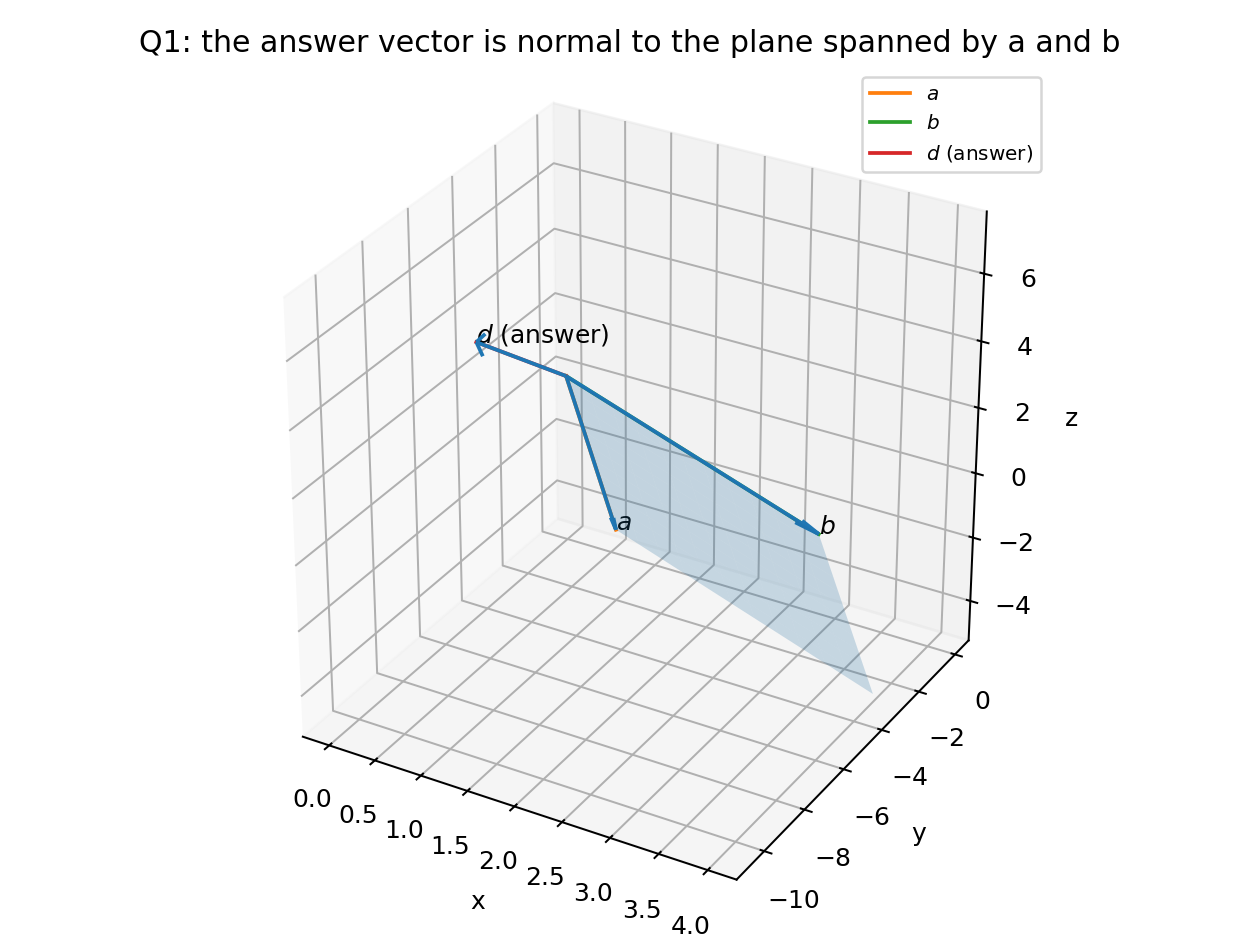
\includegraphics[width=0.96\linewidth]{figs/C12/Q01.png}
    \end{figure}

    The following code verifies the solution.

    \begin{lstlisting}[frame=single, basicstyle=\rmfamily, escapeinside={(*@}{@*)}]
(*@\makebox[\dimexpr\linewidth-2\fboxsep-2\fboxrule\relax][c]{codes/C12/Q01.py}@*)
    \end{lstlisting}


    \item
    \label{question:C12-Q05}
    \label{question-short:C12-Q05} Let $\vec a=\myvec{1\\4\\2}$, $\vec b=\myvec{3\\-2\\7}$ and $\vec c=\myvec{2\\-1\\4}$. Find $\vec d$ perpendicular to both $\vec a,\vec b$ with $\vec c\cdot\vec d=27$.

    \par
    \smallskip
    \solution

    The antisymmetric bilinear operation supplies a direction perpendicular to both prescribed vectors. Computing its determinant gives
    \begin{align*}
        \vec d & =t(\vec a\times\vec b)
    \end{align*}
    \hfill\eqref{formula:C12-Q05}

    \par
    \begin{align*}
        \vec a\times\vec b & =\myvec{32 \\-1\\-14}.
    \end{align*}

    Thus the complete perpendicular family is
    \begin{align*}
        \vec d & =t\myvec{32 \\-1\\-14}.
    \end{align*}

    The remaining scalar constraint selects the scale. First,
    \begin{align*}
        \vec c\cdot(32,-1,-14) & =2(32)+(-1)(-1)+4(-14)=64+1-56=9.
    \end{align*}

    Therefore $9t=27$, so $t=3$ and
    \begin{align*}
        \vec d & =\myvec{96 \\-3\\-42}.
    \end{align*}

    The dot products $\vec a\cdot\vec d=0$ and $\vec b\cdot\vec d=0$, together with $\vec c\cdot\vec d=27$, verify the corrected result.

    \begin{figure}[H]
        \centering
        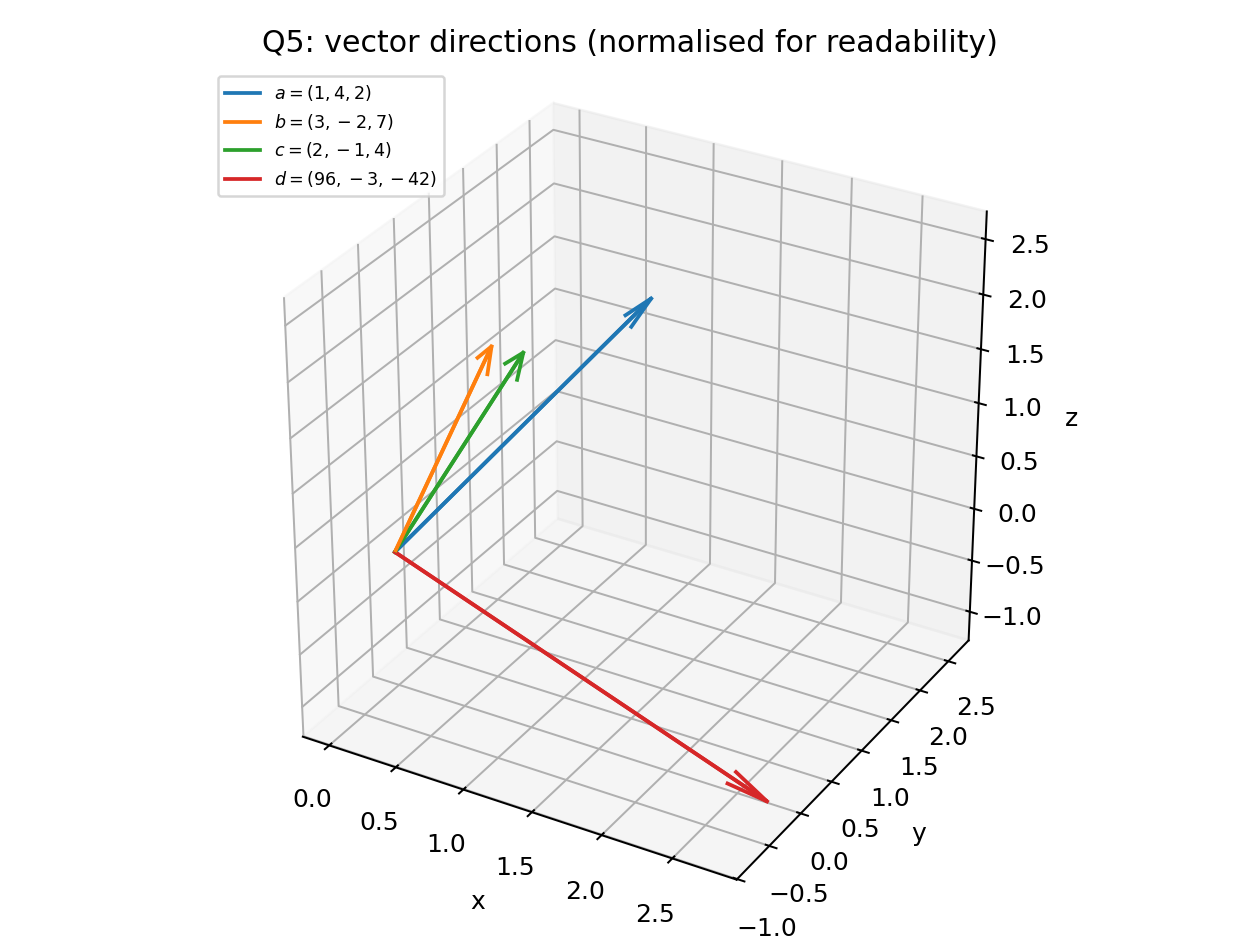
\includegraphics[width=0.96\linewidth]{figs/C12/Q05.png}
    \end{figure}

    The following code verifies the solution.

    \begin{lstlisting}[frame=single, basicstyle=\rmfamily, escapeinside={(*@}{@*)}]
(*@\makebox[\dimexpr\linewidth-2\fboxsep-2\fboxrule\relax][c]{codes/C12/Q05.py}@*)
    \end{lstlisting}


    \item
    \label{question:C12-Q06}
    \label{question-short:C12-Q06} Find the shortest distance between $\vec r=(1,2,3)+\lambda(2,3,4)$ and $\vec r=(2,4,5)+\mu(4,6,8)$.

    \par
    \smallskip
    \solution

    The direction vectors $(2,3,4)$ and $(4,6,8)$ are parallel. Choose one point on each line and form the joining vector
    \begin{align*}
        \vec v & =(2,3,4)^T,\qquad \vec w=(2,4,5)-(1,2,3)=(1,2,2)^T.
    \end{align*}

    Only the component of $\vec w$ orthogonal to the common direction contributes to the shortest distance. The projection-residual operator is
    \begin{align*}
        P_\perp & =I-\frac{\vec v\vec v^T}{\vec v^T\vec v}.
    \end{align*}
    \hfill\eqref{formula:C12-Q06}

    \par
    \begin{align*}
        d & =\|P_\perp\vec w\|=\frac{\|\vec w\times\vec v\|}{\|\vec v\|}
    \end{align*}
    \hfill\eqref{formula:C12-Q06-S01}

    \par
    Here
    \begin{align*}
        \vec w\times\vec v     & =\myvec{2   \\0\\-1}. \\
        \|\vec w\times\vec v\| & =\sqrt5.    \\
        \|\vec v\|             & =\sqrt{29}.
    \end{align*}

    Consequently,
    \begin{align*}
        d & =\sqrt{\frac5{29}}.
    \end{align*}

    The cross product is orthogonal to $\vec v$, so the residual satisfies the required projection consistency check.

    \begin{figure}[H]
        \centering
        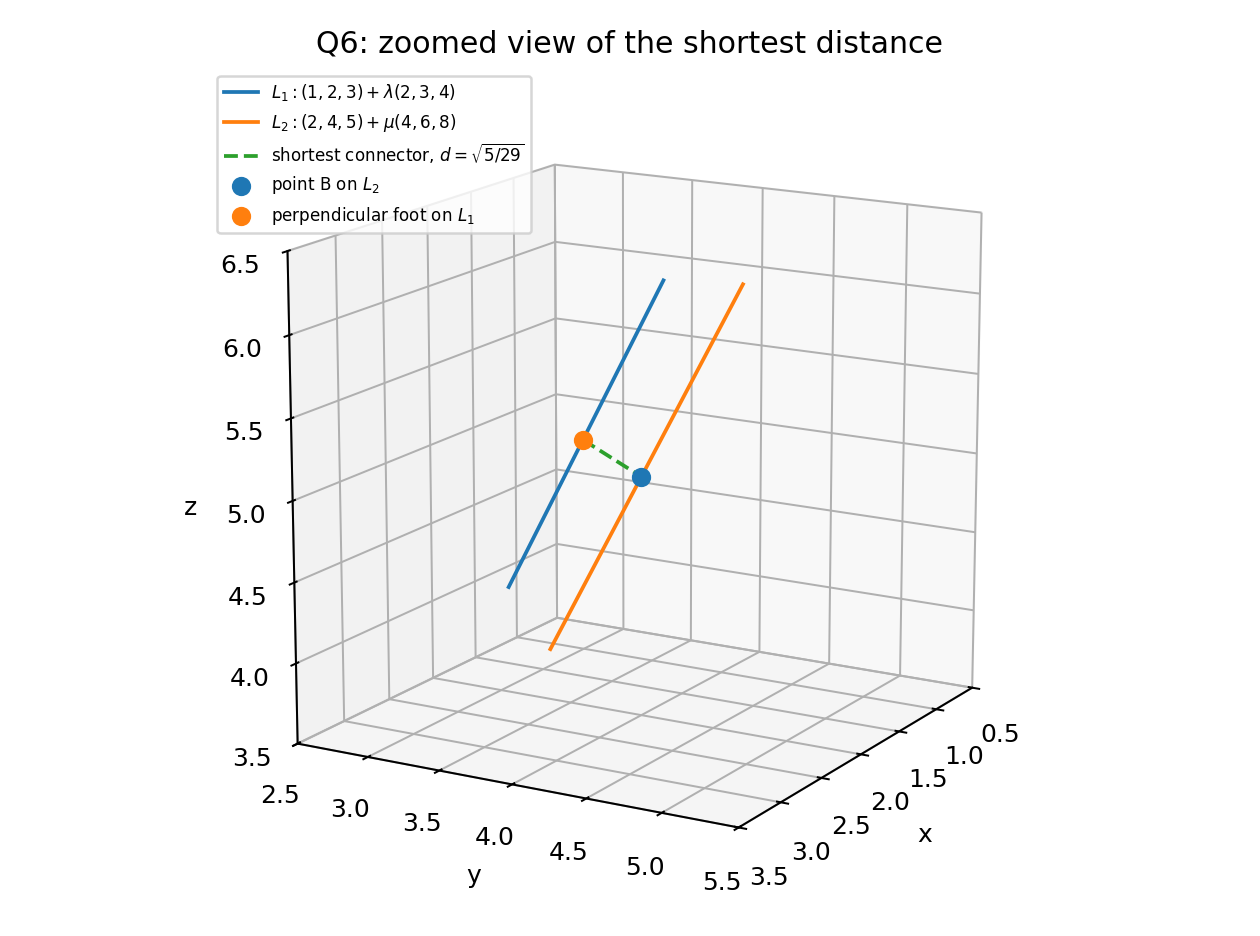
\includegraphics[width=0.96\linewidth]{figs/C12/Q06.png}
    \end{figure}

    The following code verifies the solution.

    \begin{lstlisting}[frame=single, basicstyle=\rmfamily, escapeinside={(*@}{@*)}]
(*@\makebox[\dimexpr\linewidth-2\fboxsep-2\fboxrule\relax][c]{codes/C12/Q06.py}@*)
    \end{lstlisting}


    \par
    \medskip
    \noindent\textbf{Lines and planes}
    \par
    \smallskip

    \item
    \label{question:C12-Q10}
    \label{question-short:C12-Q10} Find the plane through the intersection of $2x+y-z=3$ and $5x-3y+4z+9=0$ that is parallel to $\frac{x-1}{2}=\frac{y-3}{-4}=\frac{5-z}{-5}$.

    \par
    \smallskip
    \solution

    Let
    \begin{align*}
        P_1 & =2x+y-z-3.   \\
        P_2 & =5x-3y+4z+9.
    \end{align*}

    Every plane through the intersection line belongs to the affine pencil $P_1+\lambda P_2=0$. Its normal is
    \begin{align*}
        \vec n(\lambda) & =(2+5\lambda,\,1-3\lambda,\,-1+4\lambda).
    \end{align*}

    The direction of the given line is $\vec d=(2,-4,5)$. The required parallelism condition is
    \begin{align*}
        (\vec n_1+\lambda\vec n_2)\cdot\vec d & =0.
    \end{align*}
    \hfill\eqref{formula:C12-Q10}

    \par
    Substitution gives
    \begin{align*}
        2(2+5\lambda)-4(1-3\lambda)+5(-1+4\lambda) & =0,
    \end{align*}

    so $-5+42\lambda=0$ and $\lambda=5/42$. Multiplying the pencil by 42 yields
    \begin{align*}
        42P_1+5P_2 & =0
        \Longrightarrow 109x+27y-22z-81=0.
    \end{align*}

    The plane contains the intersection line by construction, and its normal has zero dot product with the given line direction.

    \begin{figure}[H]
        \centering
        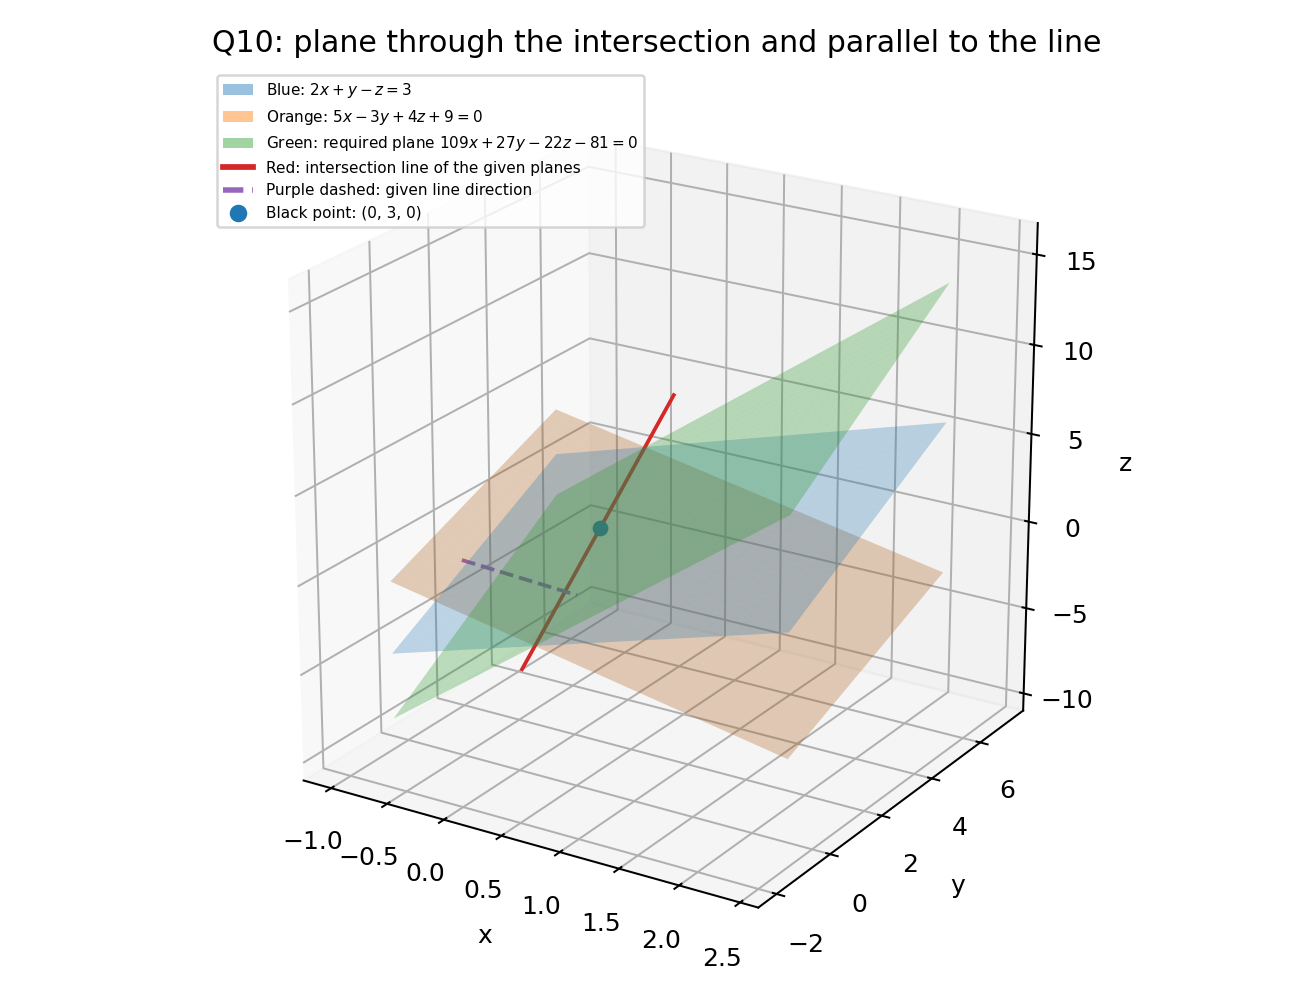
\includegraphics[width=0.96\linewidth]{figs/C12/Q10.png}
    \end{figure}

    The following code verifies the solution.

    \begin{lstlisting}[frame=single, basicstyle=\rmfamily, escapeinside={(*@}{@*)}]
(*@\makebox[\dimexpr\linewidth-2\fboxsep-2\fboxrule\relax][c]{codes/C12/Q10.py}@*)
    \end{lstlisting}


    \item
    \label{question:C12-Q15}
    \label{question-short:C12-Q15} Find where the line through $A(3,4,1)$ and $B(5,1,6)$ meets the plane through $P(2,1,2)$, $Q(3,1,0)$ and $R(4,-2,1)$.

    \par
    \smallskip
    \solution

    The two plane-edge vectors are
    \begin{align*}
        Q-P & =(1,0,-2).  \\
        R-P & =(2,-3,-1).
    \end{align*}

    Their cross product is proportional to $(2,1,1)$, so the plane equation is
    \begin{align*}
        2(x-2)+(y-1)+(z-2) & =0
        \Longrightarrow 2x+y+z=7.
    \end{align*}

    The line direction is $B-A=(2,-3,5)$. Its affine representation is
    \begin{align*}
        \vec r & =\vec A+t\vec d.
    \end{align*}
    \hfill\eqref{formula:C12-Q15}

    \par
    Thus
    \begin{align*}
        \vec r & =(3,4,1)+t(2,-3,5).
    \end{align*}

    Substitution into the plane gives
    \begin{align*}
        2(3+2t)+(4-3t)+(1+5t) & =7
        \Longrightarrow 11+6t=7
        \Longrightarrow t=-\frac23.
    \end{align*}

    The intersection point is therefore
    \begin{align*}
        & \left(\frac53,6,-\frac73\right).
    \end{align*}

    Putting this point back into $2x+y+z$ gives $10/3+6-7/3=7$, which verifies the incidence condition.

    \begin{figure}[H]
        \centering
        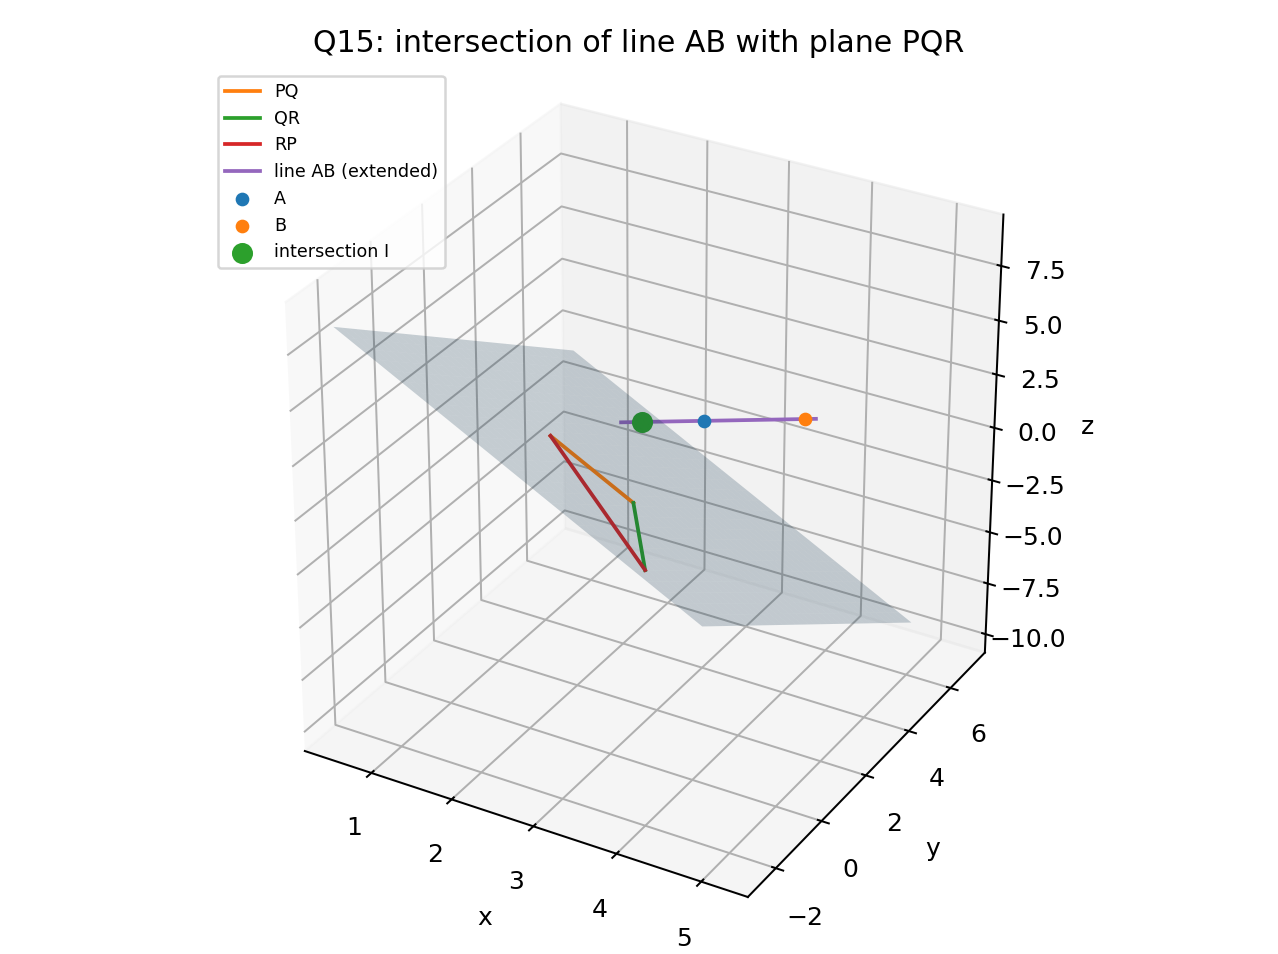
\includegraphics[width=0.96\linewidth]{figs/C12/Q15.png}
    \end{figure}

    The following code verifies the solution.

    \begin{lstlisting}[frame=single, basicstyle=\rmfamily, escapeinside={(*@}{@*)}]
(*@\makebox[\dimexpr\linewidth-2\fboxsep-2\fboxrule\relax][c]{codes/C12/Q15.py}@*)
    \end{lstlisting}


    \item
    \label{question:C12-Q25}
    \label{question-short:C12-Q25} If $y=\log\left(\frac{x}{a+bx}\right)^x$, prove that $x^3y''=(xy'-y)^2$.

    \par
    \smallskip
    \solution

    Interpret the displayed power as
    \begin{align*}
        y & =x\log\left(\frac{x}{a+bx}\right),
    \end{align*}

    on a domain where the logarithm is defined. The logarithmic derivative identity and the Euler operator $\theta=x\,d/dx$ give
    \begin{align*}
        \frac{d}{dx}\log|u| & =\frac{u'}u.
    \end{align*}
    \hfill\eqref{formula:C12-Q25}

    \par
    \begin{align*}
        \theta y-y & =xy'-y
    \end{align*}
    \hfill\eqref{formula:C12-Q25-S01}

    \par
    Differentiate $y$ explicitly:
    \begin{align*}
        y' & =\log\left(\frac{x}{a+bx}\right)+x\left(\frac1x-\frac b{a+bx}\right)
        =\log\left(\frac{x}{a+bx}\right)+\frac a{a+bx}.
    \end{align*}

    Differentiating once more,
    \begin{align*}
        y'' & =\frac1x-\frac b{a+bx}-\frac{ab}{(a+bx)^2}
        =\frac{a^2}{x(a+bx)^2}.
    \end{align*}

    The Euler combination simplifies without the logarithm:
    \begin{align*}
        xy'-y & =x\frac a{a+bx}=\frac{ax}{a+bx}.
    \end{align*}

    Squaring it and comparing with $y''$ gives
    \begin{align*}
        (xy'-y)^2 & =\frac{a^2x^2}{(a+bx)^2}=x^3\frac{a^2}{x(a+bx)^2}=x^3y''.
    \end{align*}

    Hence
    \begin{align*}
        x^3y'' & =(xy'-y)^2.
    \end{align*}


    \par
    \medskip
    \noindent\textbf{Matrices and determinants}
    \par
    \smallskip

    \item
    \label{question:C12-Q28}
    \label{question-short:C12-Q28} If $A=\myvec{\cos\theta&\sin\theta\\\sin\theta&\cos\theta}$, find $\det(A^n)$ for natural $n$.

    \par
    \smallskip
    \solution

    The symmetric matrix has eigenvectors $q_+=(1,1)^T$ and $q_-=(1,-1)^T$. Their eigenvalues are
    \begin{align*}
        \lambda_+ & =\cos\theta+\sin\theta. \\
        \lambda_- & =\cos\theta-\sin\theta.
    \end{align*}

    $\det A=\lambda_+\lambda_-$ and raises each eigenvalue to the $n$th power. Using the determinant-power identity,
    \begin{align*}
        \det(A^n) & =(\det A)^n.
    \end{align*}
    \hfill\eqref{formula:C12-Q28}

    \par
    We obtain
    \begin{align*}
        \det(A^n) & =(\lambda_+\lambda_-)^n
        =\bigl((\cos\theta+\sin\theta)(\cos\theta-\sin\theta)\bigr)^n
        =(\cos2\theta)^n.
    \end{align*}


    \item
    \label{question:C12-Q30}
    \label{question-short:C12-Q30} Find the inverse of $\myvec{0&1&2\\1&2&3\\3&1&0}$ using elementary row operations.

    \par
    \smallskip
    \solution

\[
A=\myvec{
0&1&2\\
1&2&3\\
3&1&0
}
\]

\[
\myvec{
0&1&2&\big|&1&0&0\\
1&2&3&\big|&0&1&0\\
3&1&0&\big|&0&0&1
}
\]

\[
R_1\leftrightarrow R_2
\]

\[
\myvec{
1&2&3&\big|&0&1&0\\
0&1&2&\big|&1&0&0\\
3&1&0&\big|&0&0&1
}
\]

\[
R_3\rightarrow R_3-3R_1
\]

\[
\myvec{
1&2&3&\big|&0&1&0\\
0&1&2&\big|&1&0&0\\
0&-5&-9&\big|&0&-3&1
}
\]

\[
R_3\rightarrow R_3+5R_2
\]

\[
\myvec{
1&2&3&\big|&0&1&0\\
0&1&2&\big|&1&0&0\\
0&0&1&\big|&5&-3&1
}
\]

\[
R_2\rightarrow R_2-2R_3
\]

\[
\myvec{
1&2&3&\big|&0&1&0\\
0&1&0&\big|&-9&6&-2\\
0&0&1&\big|&5&-3&1
}
\]

\[
R_1\rightarrow R_1-3R_3
\]

\[
\myvec{
1&2&0&\big|&-15&10&-3\\
0&1&0&\big|&-9&6&-2\\
0&0&1&\big|&5&-3&1
}
\]

\[
R_1\rightarrow R_1-2R_2
\]

\[
\myvec{
1&0&0&\big|&3&-2&1\\
0&1&0&\big|&-9&6&-2\\
0&0&1&\big|&5&-3&1
}
\]

\[
A^{-1}=
\myvec{
3&-2&1\\
-9&6&-2\\
5&-3&1
}
\]

\[
\begin{aligned}
AA^{-1}
&=
\myvec{
0&1&2\\
1&2&3\\
3&1&0
}
\myvec{
3&-2&1\\
-9&6&-2\\
5&-3&1
}\\[6pt]
&=
\myvec{
1&0&0\\
0&1&0\\
0&0&1
}\\
&=I
\end{aligned}
\]


    The following code verifies the solution.

    \begin{lstlisting}[frame=single, basicstyle=\rmfamily, escapeinside={(*@}{@*)}]
(*@\makebox[\dimexpr\linewidth-2\fboxsep-2\fboxrule\relax][c]{codes/C12/Q30.py}@*)
    \end{lstlisting}



    \item
    \label{question:C12-Q48}
    \label{question-short:C12-Q48} Discuss continuity and differentiability of $f(x)=|x|+|x-1|$ on $(-1,2)$.

    \par
    \smallskip
    \solution

    The absolute-value characteristic changes branch at $x=0$ and $x=1$. Resolving the signs gives
    \begin{align*}
        f(x) & =|x|+|x-1|=
        \begin{cases}1-2x,&-1<x<0,\\1,&0\le x<1,\\2x-1,&1\le x<2.
        \end{cases}
    \end{align*}

    At the first breakpoint,
    \begin{align*}
        \lim_{x\to0^-}f(x) & =1=f(0)=\lim_{x\to0^+}f(x),
    \end{align*}

    and at the second,
    \begin{align*}
        \lim_{x\to1^-}f(x) & =1=f(1)=\lim_{x\to1^+}f(x).
    \end{align*}

    Thus the function is continuous throughout $(-1,2)$. Its one-sided derivatives are
    \begin{align*}
        f'_-(0) & =-2. \\
        f'_+(0) & =0.  \\
        f'_-(1) & =0.  \\
        f'_+(1) & =2.
    \end{align*}

    The slopes disagree at both breakpoints, so f is not differentiable at 0 or 1, but
is differentiable elsewhere.


	\begin{figure}[H]
        \centering
        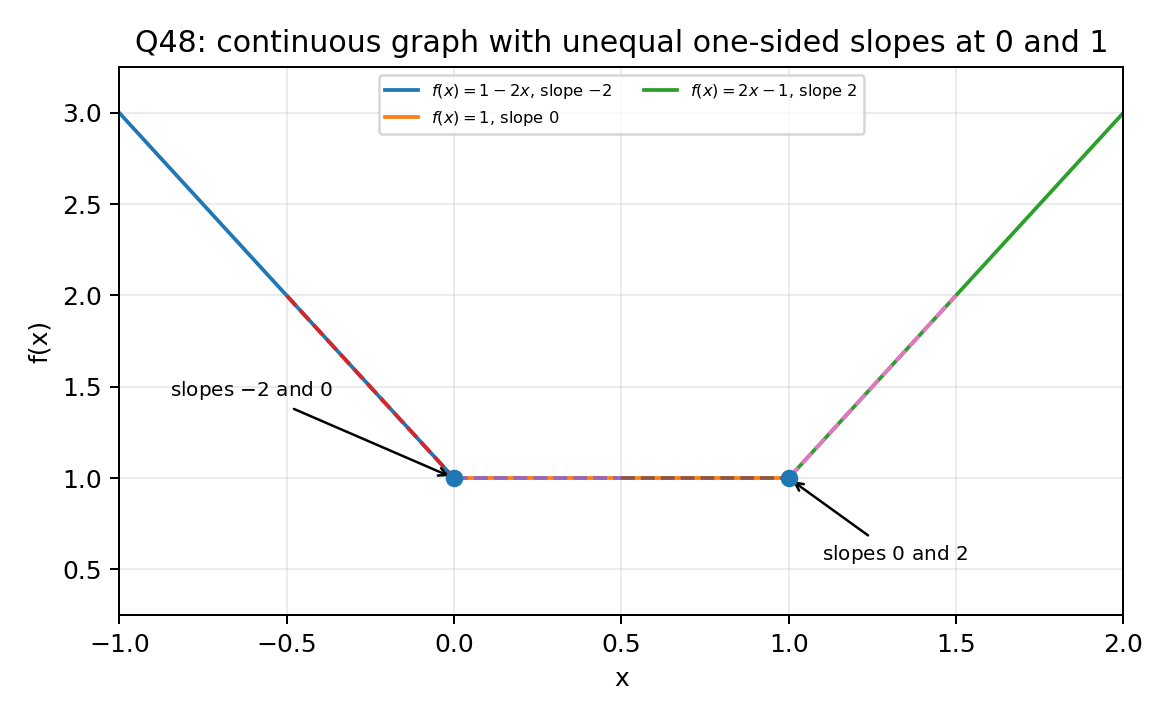
\includegraphics[width=0.92\linewidth]{figs/C12/Q48.png}
    \end{figure}

    The following code verifies the solution.

    \begin{lstlisting}[frame=single, basicstyle=\rmfamily, escapeinside={(*@}{@*)}]
(*@\makebox[\dimexpr\linewidth-2\fboxsep-2\fboxrule\relax][c]{codes/C12/Q48.py}@*)
    \end{lstlisting}


    \item
    \label{question:C12-Q49}
    \label{question-short:C12-Q49} On $\mathbb R$, define $(a,b)\in R$ when $a-b+\sqrt3$ is irrational. Determine whether $R$ is reflexive, symmetric and transitive.

    \par
    \smallskip
    \solution

    Write the relation as the predicate $R(a,b)$: the number $a-b+\sqrt3$ must lie outside $\mathbb Q$. Its defining condition is
    \begin{align*}
        R(a,b)\Longleftrightarrow a-b+\sqrt3\text{ is irrational}.
    \end{align*}

    For reflexivity, $a-a+\sqrt3=\sqrt3$ is irrational, so $R(a,a)$ holds for every $a$. Symmetry fails: with $(a,b)=(\sqrt3,0)$, the forward expression is $2\sqrt3$ (irrational), but the reversed expression is $0$ (rational). Transitivity fails for
    \begin{align*}
        a & =0.                \\
        b & =\frac{\sqrt3}{2}. \\
        c & =\sqrt3.
    \end{align*}

    Both $a-b+\sqrt3=\sqrt3/2$ and $b-c+\sqrt3=\sqrt3/2$ are irrational, while $a-c+\sqrt3=0$. Therefore
    \begin{align*}
        R\text{ is reflexive, but neither symmetric nor transitive}.
    \end{align*}


    \par
    \medskip
    \noindent\textbf{Algebraic structures}
    \par
    \smallskip

    \item
    \label{question:C12-Q50}
    \label{question-short:C12-Q50} On $\mathbb R\times\mathbb R$, define $(a,b)*(c,d)=(a+c,b+d)$. Prove commutativity and associativity, and find the identity and the inverse of $(3,-5)$.

    \par
    \smallskip
    \solution

    The operation is coordinatewise addition, so it is closed on $\mathbb R^2$. Its defining law is
    \begin{align*}
        (a,b)*(c,d) & =(a+c,b+d).
    \end{align*}
    \hfill\eqref{formula:C12-Q50}

    \par
    For associativity,
    \begin{align*}
        ((a,b)*(c,d))*(e,f) & =(a+c+e,b+d+f)
        =(a,b)*((c,d)*(e,f)).
    \end{align*}
    \hfill\eqref{formula:C12-Q50-F01}

    \par
    For commutativity,
    \begin{align*}
        (a,b)*(c,d) & =(a+c,b+d)=(c+a,d+b)=(c,d)*(a,b).
    \end{align*}
    \hfill\eqref{formula:C12-Q50-F02}

    \par
    The identity is $(0,0)$, and the inverse of $(3,-5)$ solves
    \begin{align*}
        (3,-5)*(u,v) & =(3+u,-5+v)=(0,0),
    \end{align*}

    so it is $(-3,5)$. Thus the structure is an Abelian group and
    \begin{align*}
        e & =(0,0),\qquad (3,-5)^{-1}=(-3,5).
    \end{align*}


    \item
    \label{question:C12-Q51}
    \label{question-short:C12-Q51} On $\{0,1,2,3,4,5,6\}$ define $a*b=a+b$ if $a+b<7$, and $a*b=a+b-7$ otherwise. Give the operation table and show that 0 is the identity and $7-a$ is the inverse for nonzero $a$.

    \par
    \smallskip
    \solution

    The piecewise definition is addition modulo $7$:
    \begin{align*}
        a*b & =(a+b)\bmod 7.
    \end{align*}
    \hfill\eqref{formula:C12-Q51}

    \par
    The Cayley table is
    \begin{align*}
        \begin{array}{c|rrrrrrr}* & 0 & 1 & 2 & 3 & 4 & 5 & 6 \\\hline
            0            & 0 & 1 & 2 & 3 & 4 & 5 & 6 \\1&1&2&3&4&5&6&0\\2&2&3&4&5&6&0&1\\3&3&4&5&6&0&1&2\\4&4&5&6&0&1&2&3\\5&5&6&0&1&2&3&4\\6&6&0&1&2&3&4&5
        \end{array}
    \end{align*}

    The first row and column show $0*a=a*0=a$. For nonzero $a$, the residue $7-a$ lies in the set and
    \begin{align*}
        a*(7-a) & =a+7-a\equiv0\pmod7.
    \end{align*}
    \hfill\eqref{formula:C12-Q51-F02}

    \par
    Since $7$ is prime, every nonzero residue generates the cyclic group $\mathbb Z_7$. Therefore
    \begin{align*}
        0\text{ is the identity and }a^{-1} & =7-a\pmod7.
    \end{align*}


    \item
    \label{question:C12-Q52}
    \label{question-short:C12-Q52} Find any point of discontinuity of $f(x)=x-|x-x^2|$, $x\in[-1,1]$.

    \par
    \smallskip
    \solution

    Factor the expression inside the absolute value:
    \begin{align*}
        x-x^2 & =x(1-x).
    \end{align*}
    \hfill\eqref{formula:C12-Q52}

    \par
    On $[-1,1]$, this quantity is nonnegative for $0\le x\le1$ and nonpositive for $-1\le x\le0$. The piecewise nonlinear map is therefore
    \begin{align*}
        f(x) & =
        \begin{cases}2x-x^2,&-1\le x\le0,\\x^2,&0\le x\le1.
        \end{cases}
    \end{align*}

    At the switching point, both branches give $f(0)=0$. Moreover,
    \begin{align*}
        \lim_{x\to0^-}(2x-x^2) & =0=f(0)=\lim_{x\to0^+}x^2.
    \end{align*}

    Thus there is no discontinuity on the domain.

    \begin{align*}
        \text{there is no point of discontinuity on }[-1,1].
    \end{align*}

    \begin{figure}[H]
        \centering
        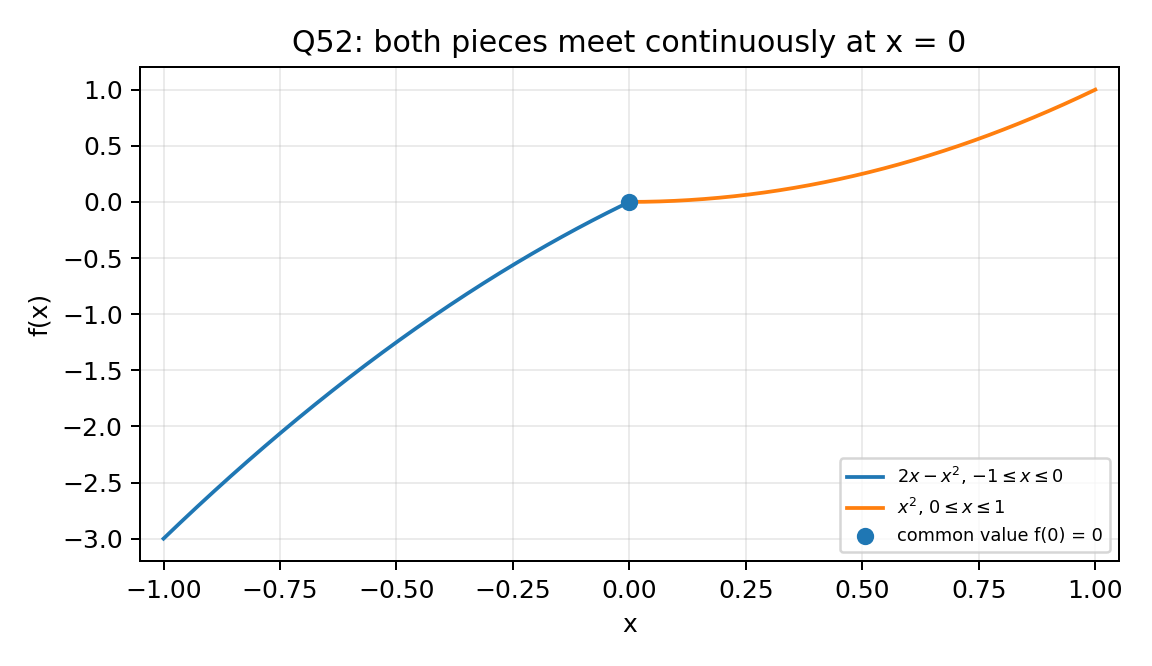
\includegraphics[width=0.92\linewidth]{figs/C12/Q52.png}
    \end{figure}

    The following code verifies the solution.

    \begin{lstlisting}[frame=single, basicstyle=\rmfamily, escapeinside={(*@}{@*)}]
(*@\makebox[\dimexpr\linewidth-2\fboxsep-2\fboxrule\relax][c]{codes/C12/Q52.py}@*)
    \end{lstlisting}


    \item
    \label{question:C12-Q53}
    \label{question-short:C12-Q53} A man steps forward with probability $0.4$ and backward with probability $0.6$. Find the probability that after 5 steps he is one step away from his starting point.

    \par
    \smallskip
    \solution


    After five steps, displacement $+1$ requires three forward and two backward steps, while displacement $-1$ requires two forward and three backward steps.
    \begin{align*}
        P(|D|=1) & =\binom53(0.4)^3(0.6)^2+\binom52(0.4)^2(0.6)^3.
    \end{align*}
    \hfill\eqref{formula:C12-Q53}\par

    Numerically,
    \begin{align*}
        \binom53(0.064)(0.36)+\binom52(0.16)(0.216) & =0.3456+0.2304=0.576.
    \end{align*}

    The two cases are disjoint and exhaust the requested one-step displacement events.

    \begin{figure}[H]
        \centering
        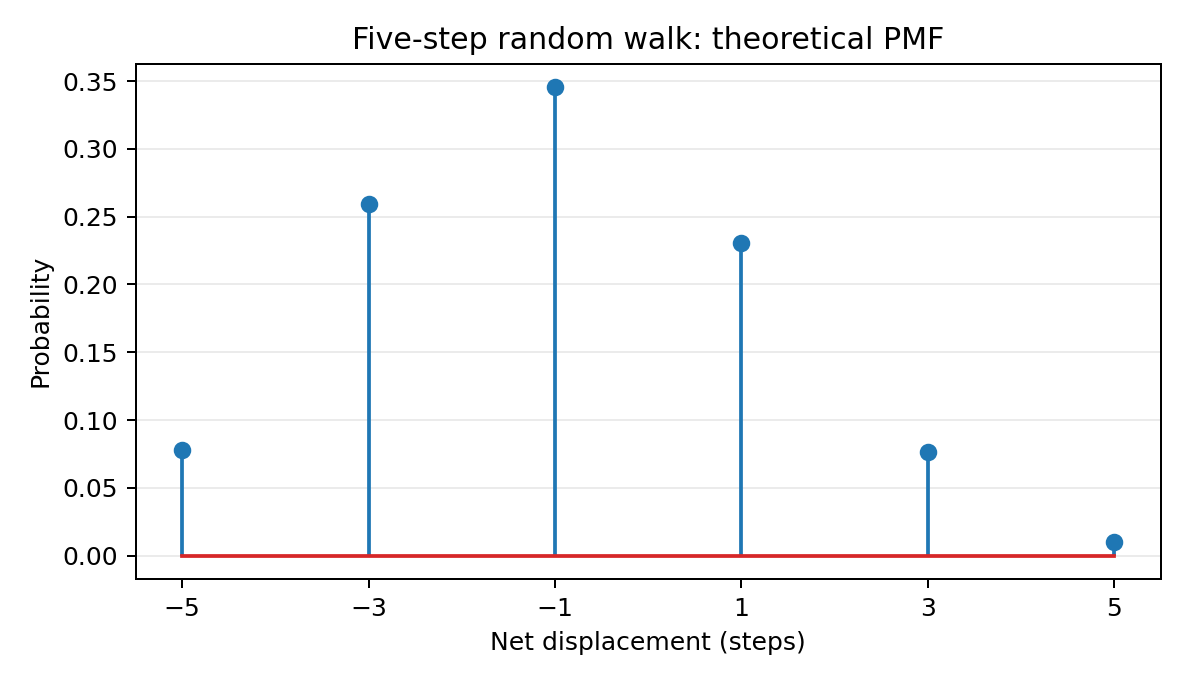
\includegraphics[width=0.92\linewidth]{figs/C12/Q53.png}
    \end{figure}

    The following code verifies the solution.

    \begin{lstlisting}[frame=single, basicstyle=\rmfamily, escapeinside={(*@}{@*)}]
(*@\makebox[\dimexpr\linewidth-2\fboxsep-2\fboxrule\relax][c]{codes/C12/Q53.py}@*)
    \end{lstlisting}


    \item
    \label{question:C12-Q54}
    \label{question-short:C12-Q54} A girl throws a die. If it shows 1 or 2, she tosses a coin three times; otherwise she tosses it once. Given that exactly one tail was obtained, find the probability that the die showed 3, 4, 5 or 6.

    \par
    \smallskip
    \solution

    Let $H_1$ denote die outcomes $1$ or $2$, $H_2$ denote outcomes $3,4,5,6$, and let $E$ be the event of exactly one tail. Then
    \begin{align*}
        P(H_1) & =\frac13. \\
        P(H_2) & =\frac23.
    \end{align*}

    Under $H_1$, exactly one tail in three tosses has likelihood $3(1/2)^3=3/8$; under $H_2$, exactly one tail in one toss has likelihood $1/2$. Bayes' rule is
    \begin{align*}
        P(H_2\mid E) & =\frac{P(E\mid H_2)P(H_2)}{P(E)}.
    \end{align*}
    \hfill\eqref{formula:C12-Q54}

    \par
    The evidence probability is
    \begin{align*}
        P(E) & =\frac38\cdot\frac13+\frac12\cdot\frac23=\frac18+\frac13=\frac{11}{24}.
    \end{align*}

    Therefore
    \begin{align*}
        P(H_2\mid E) & =\frac{(1/2)(2/3)}{11/24}=\frac{1/3}{11/24}=\frac8{11}.
    \end{align*}

        \begin{figure}[H]
        \centering
        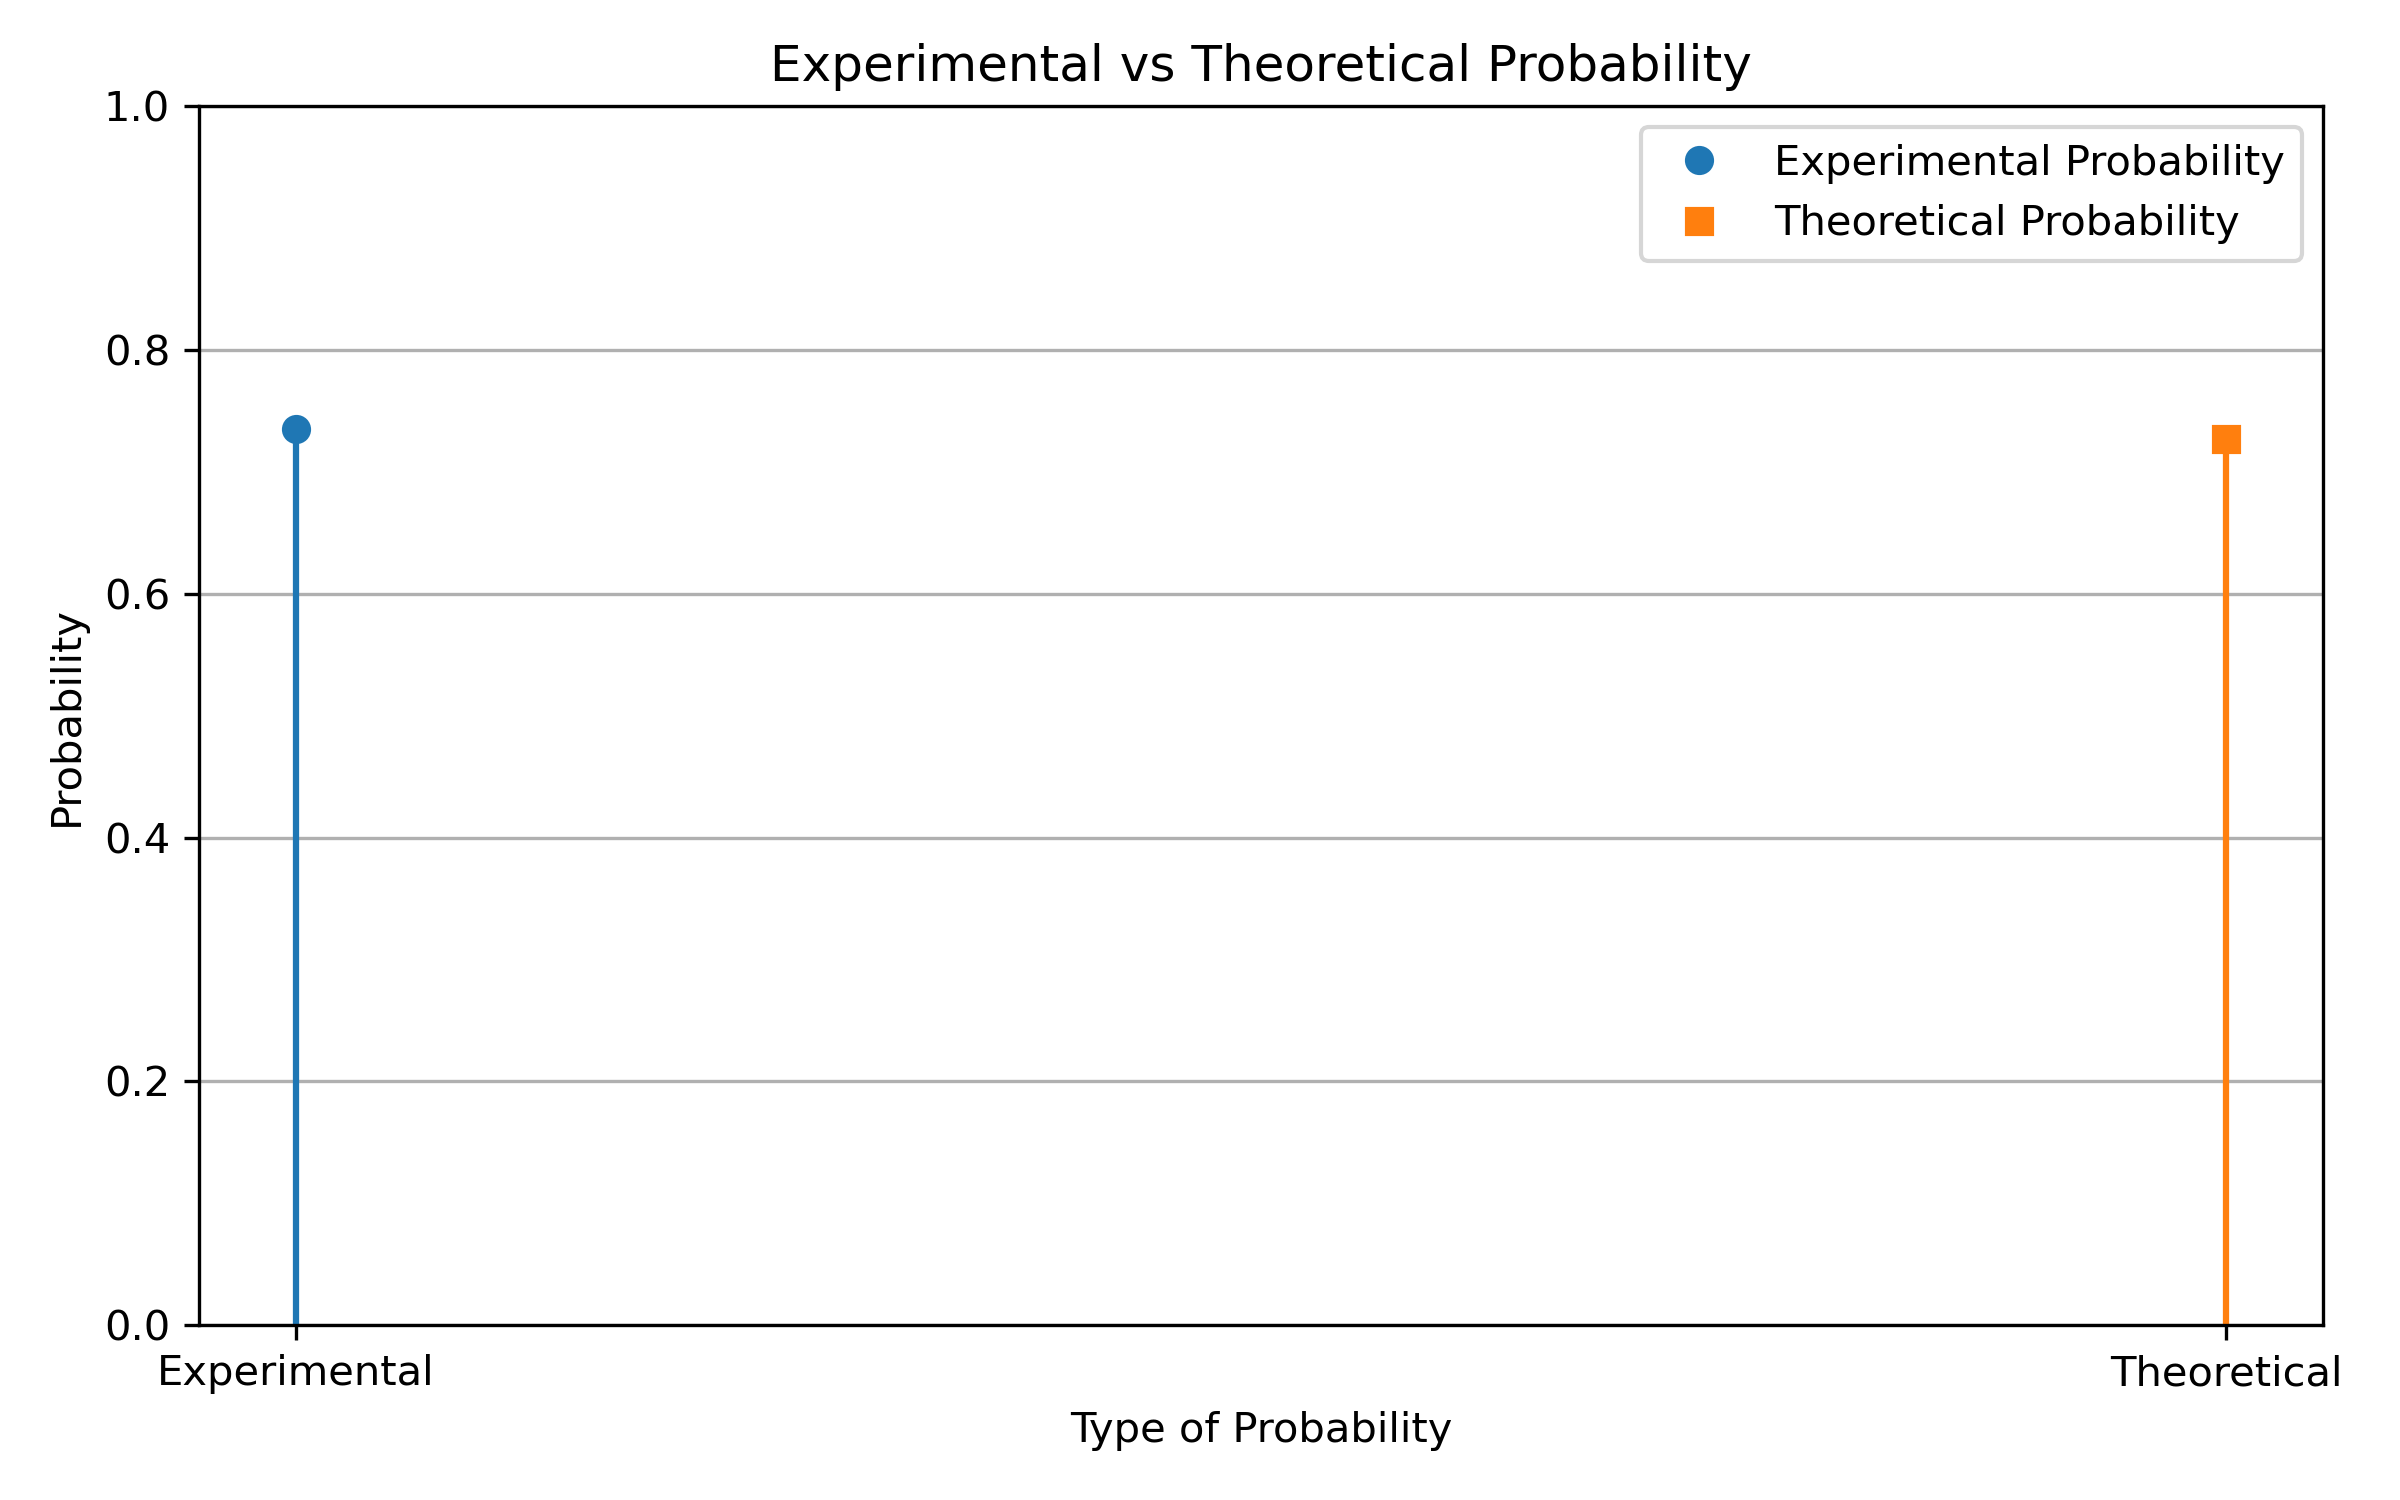
\includegraphics[width=0.92\linewidth]{figs/C12/Q54.png}
    \end{figure}

    The following code generates 10,000 outcomes.
        \begin{lstlisting}[frame=single, basicstyle=\rmfamily, escapeinside={(*@}{@*)}]
(*@\makebox[\dimexpr\linewidth-2\fboxsep-2\fboxrule\relax][c]{codes/C12/Q54/Q54.c}@*)
    \end{lstlisting}

    The following code verifies the solution.
        \begin{lstlisting}[frame=single, basicstyle=\rmfamily, escapeinside={(*@}{@*)}]
(*@\makebox[\dimexpr\linewidth-2\fboxsep-2\fboxrule\relax][c]{codes/C12/Q54/Q54.py}@*)
    \end{lstlisting}

    \item
    \label{question:C12-Q55}
    \label{question-short:C12-Q55} An urn contains 5 red and 2 black balls. Two balls are drawn without replacement. Let $X$ be the number of black balls. State its possible values and find its mean and variance.

    \par
    \smallskip
    \solution

    Without replacement, $X$ has a hypergeometric distribution with population size $N=7$, black count $K=2$, and sample size $n=2$. Thus $X\in\{0,1,2\}$ and the probability mass is
    \begin{align*}
        P(X=0) & =\frac{10}{21}. \\
        P(X=1) & =\frac{10}{21}. \\
        P(X=2) & =\frac1{21}.
    \end{align*}

    The three probabilities are
    \begin{align*}
        P(X=0) & =\frac{10}{21},\qquad P(X=1)=\frac{10}{21},\qquad P(X=2)=\frac1{21}.
    \end{align*}

    The probability-generating function method uses
    \begin{align*}
        G_X(z) & =\sum_xP(X=x)z^x.
    \end{align*}
    \hfill\eqref{formula:C12-Q55}

    \par
    Here
    \begin{align*}
        G_X(z)  & =\frac{10+10z+z^2}{21}. \\
        G'_X(1) & =\frac{12}{21}=\frac47.
    \end{align*}

    and
    \begin{align*}
        G''_X(1) & =\frac2{21}=E[X(X-1)].
    \end{align*}

    Consequently,
    \begin{align*}
        E[X^2]                & =E[X(X-1)]+E[X]=\frac2{21}+\frac47=\frac{20}{21},          \\
        \operatorname{Var}(X) & =E[X^2]-E[X]^2=\frac{20}{21}-\frac{16}{49}=\frac{50}{147}.
    \end{align*}

    \begin{figure}[H]
        \centering
        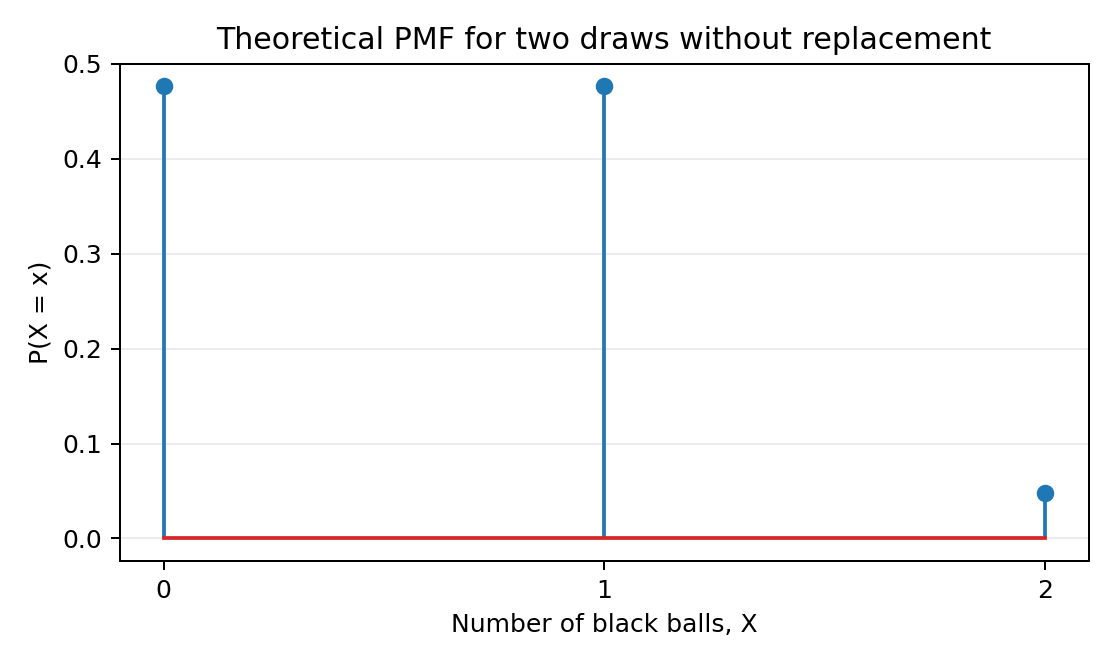
\includegraphics[width=0.92\linewidth]{figs/C12/Q55.png}
    \end{figure}

    The following code verifies the solution.

    \begin{lstlisting}[frame=single, basicstyle=\rmfamily, escapeinside={(*@}{@*)}]
(*@\makebox[\dimexpr\linewidth-2\fboxsep-2\fboxrule\relax][c]{codes/C12/Q55.py}@*)
    \end{lstlisting}


    \item
    \label{question:C12-Q56}
    \label{question-short:C12-Q56} In 3 trials of a binomial distribution, the probability of exactly 2 successes is 9 times the probability of 3 successes. Find the success probability.

    \par
    \smallskip
    \solution

    For three independent trials with success probability $p$,
    \begin{align*}
	     P(X=x)=\binom3xp^x(1-p)^{(3-x)}.
    \end{align*}
    \hfill\eqref{formula:C12-Q56}

    \par
    
    \begin{align*}
        P(X=2) & =\binom32p^2(1-p)=3p^2(1-p). \\
        P(X=3) & =p^3.
    \end{align*}

    The given relation produces
    \begin{align*}
        3p^2(1-p) & =9p^3
        \Longrightarrow 3p^2(1-4p)=0.
    \end{align*}

    Both roots are admissible probabilities in $[0,1]$:
    \begin{align*}
        p & =0\quad\text{or}\quad p=\frac14.
    \end{align*}

    The $p=0$ case makes both probabilities zero, so it is retained as an edge case rather than divided away.

    The following code verifies the solution.

    \begin{lstlisting}[frame=single, basicstyle=\rmfamily, escapeinside={(*@}{@*)}]
(*@\makebox[\dimexpr\linewidth-2\fboxsep-2\fboxrule\relax][c]{codes/C12/Q56.py}@*)
    \end{lstlisting}


    \item
    \label{question:C12-Q57}
    \label{question-short:C12-Q57} An urn contains 3 red and 5 black balls. A ball is drawn, its colour recorded and returned, and 2 more balls of that colour are added. Then two balls are drawn without replacement. Find the probability both are red.

    \par
    \smallskip
    \solution

    Condition on the colour of the reinforced first draw. The initial state is $(R,B)=(3,5)$, so the branch probabilities are $3/8$ and $5/8$. After a red first draw the state is $(5,5)$; after a black first draw it is $(3,7)$. The law of total probability is
    \begin{align*}
        P(E) & =\sum_iP(E\mid S_i)P(S_i).
    \end{align*}
    \hfill\eqref{formula:C12-Q57}

    \par
    For the red branch,
    \begin{align*}
        P(RR\mid R_1) & =\frac5{10}\frac4{9}=\frac29.
    \end{align*}

    For the black branch,
    \begin{align*}
        P(RR\mid B_1) & =\frac3{10}\frac2{9}=\frac1{15}.
    \end{align*}

    Combining the mutually exclusive branches,
    \begin{align*}
        P(RR) & =\frac38\frac29+\frac58\frac1{15}
        =\frac1{12}+\frac1{24}=\frac18.
    \end{align*}

    The state update is applied before the two final draws, preserving the reinforcement dependence.

    The following code verifies the solution.

    \begin{lstlisting}[frame=single, basicstyle=\rmfamily, escapeinside={(*@}{@*)}]
(*@\makebox[\dimexpr\linewidth-2\fboxsep-2\fboxrule\relax][c]{codes/C12/Q57.py}@*)
    \end{lstlisting}


    \par
    \medskip
    \noindent\textbf{Optimization}
    \par
    \smallskip

    \item
    \label{question:C12-Q59}
    \label{question-short:C12-Q59} Solve graphically: minimise $z=3x+5y$ subject to $x+2y\ge10$, $x+y\ge6$, $3x+y\ge8$, $x,y\ge0$.

    \par
    \smallskip
    \solution

    The feasible region is the intersection of three half-planes in the first quadrant. Its relevant corner is obtained by making the first two constraints active:
    \begin{align*}
        x+2y & =10. \\
        x+y  & =6.
    \end{align*}

    The objective admits the duality decomposition
    \begin{align*}
        3x+5y & =2(x+2y)+(x+y).
    \end{align*}

    For every feasible point this gives $3x+5y\ge2(10)+6=26$. At $(2,4)$ equality holds, and the third constraint is satisfied because $3(2)+4=10\ge8$. Therefore the graphical minimum is
    \begin{align*}
        (x,y) & =(2,4),\qquad z_{\min}=3(2)+5(4)=26.
    \end{align*}

    Equivalently, the dual certificate $(u,v,w)=(2,1,0)$ is feasible and has objective value $20+6=26$, confirming global optimality.

    \begin{figure}[H]
        \centering
        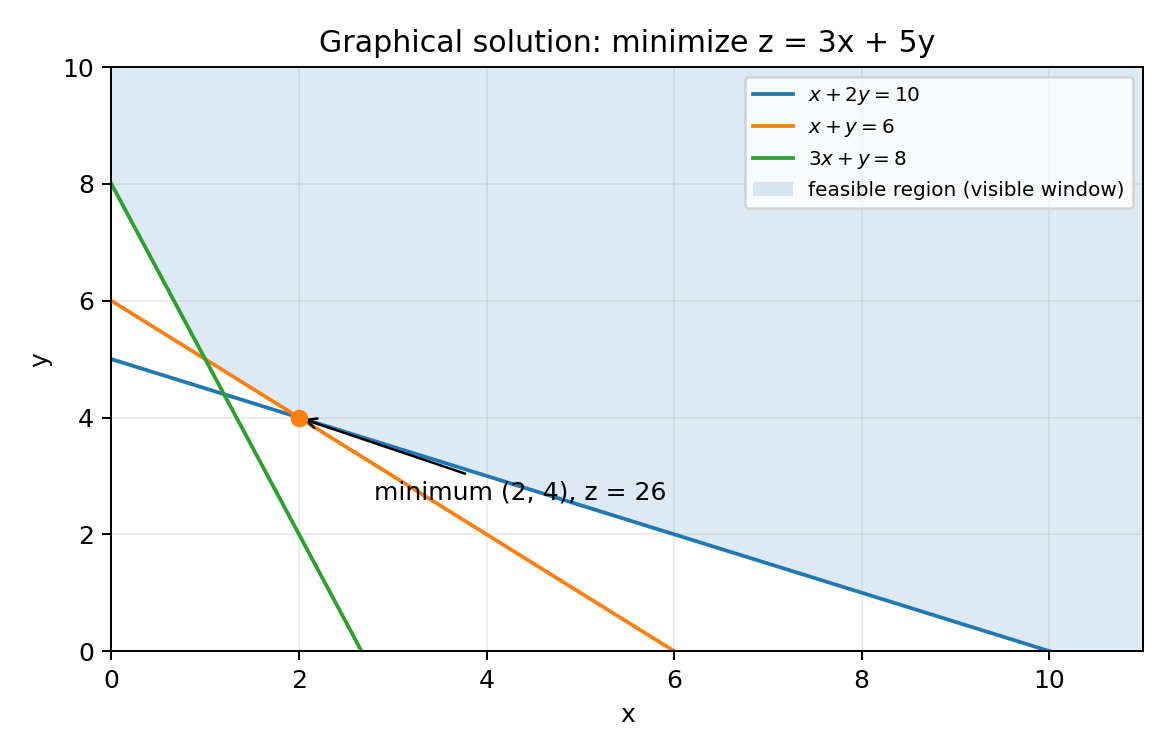
\includegraphics[width=0.92\linewidth]{figs/C12/Q59.png}
    \end{figure}

    The following code verifies the solution.

    \begin{lstlisting}[frame=single, basicstyle=\rmfamily, escapeinside={(*@}{@*)}]
(*@\makebox[\dimexpr\linewidth-2\fboxsep-2\fboxrule\relax][c]{codes/C12/Q59.py}@*)
    \end{lstlisting}


    \item
    \label{question:C12-Q60}
    \label{question-short:C12-Q60} A dealer has Rs. 57,600 and space for at most 20 sewing machines. An electronic machine costs Rs. 3600 and earns Rs. 220 profit; a manual machine costs Rs. 2400 and earns Rs. 180 profit. How should he invest to maximise profit?

    \par
    \smallskip
    \solution

    Purchasing \(e\) electronic machines costs Rs. \(3600e\), while purchasing \(m\) manual machines costs Rs. \(2400m\).The total expenditure must not exceed Rs. 57,600.

Hence, $3e+2m\le48$, $e+m\le20$, $e\ge0$ and $m\ge0$
    \[
\vec{x}=\myvec{
e\\
m
},\qquad
\vec{c}=\myvec{
220\\
180
},\qquad
\vec{b}=\myvec{
48\\
20
}
\]

\[
A=\myvec{
3&2\\
1&1
}
\]

\[
\text{Maximise } P=\vec{c}^{\,T}\vec{x}
\]

\[
A\vec{x}\leq\vec{b},
\qquad
\vec{x}\geq\vec{0}
\]

\[
\begin{aligned}
P
&=\vec{c}^{\,T}\vec{x}\\
&=\myvec{220&180}
\myvec{
e\\
m
}
\end{aligned}
\]

\[
\myvec{
3&2\\
1&1
}
\myvec{
e\\
m
}
\leq
\myvec{
48\\
20
}
\]

\[
\vec{y}=\myvec{
u\\
v
}
\]

\[
\text{Minimise } D=\vec{b}^{\,T}\vec{y}
\]

\[
A^T\vec{y}\geq\vec{c},
\qquad
\vec{y}\geq\vec{0}
\]

\[
\myvec{
3&1\\
2&1
}
\myvec{
u\\
v
}
\geq
\myvec{
220\\
180
}
\]

\[
\myvec{
3&1\\
2&1
}
\myvec{
u\\
v
}
=
\myvec{
220\\
180
}
\]

\[
\begin{aligned}
3u+v&=220\\
2u+v&=180
\end{aligned}
\]

\[
u=40,\qquad v=100
\]

\[
\vec{y}=\myvec{
40\\
100
}
\]

\[
\begin{aligned}
D
&=\vec{b}^{\,T}\vec{y}\\
&=\myvec{48&20}
\myvec{
40\\
100
}\\
&=3920
\end{aligned}
\]

\[
A\vec{x}=\vec{b}
\]

\[
\myvec{
3&2\\
1&1
}
\myvec{
e\\
m
}
=
\myvec{
48\\
20
}
\]

\[
\vec{x}=\myvec{
8\\
12
}
\]

\[
\begin{aligned}
P
&=\vec{c}^{\,T}\vec{x}\\
&=\myvec{220&180}
\myvec{
8\\
12
}\\
&=3920
\end{aligned}
\]

\[
P=D=3920
\]

\[
\vec{x}=\myvec{
8\\
12
},
\qquad
P_{\max}=\text{Rs. }3920
\]

    \begin{figure}[H]
        \centering
        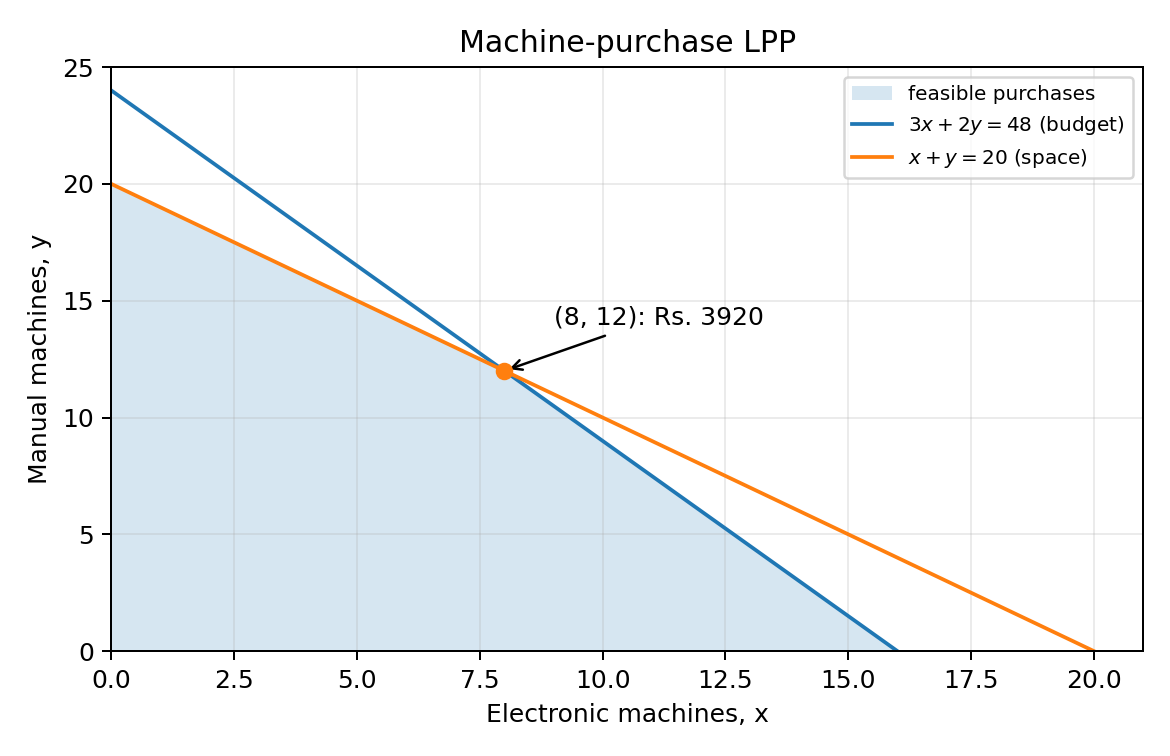
\includegraphics[width=0.92\linewidth]{figs/C12/Q60.png}
    \end{figure}


    The following code verifies the solution.

    \begin{lstlisting}[frame=single, basicstyle=\rmfamily, escapeinside={(*@}{@*)}]
(*@\makebox[\dimexpr\linewidth-2\fboxsep-2\fboxrule\relax][c]{codes/C12/Q60.py}@*)
    \end{lstlisting}

    \end{enumerate}


